\documentclass[10pt]{article}
\usepackage[OT1]{fontenc}
\usepackage[utf8]{inputenc}
\bibliographystyle{plain}

\usepackage[ruled,vlined]{algorithm2e}
\usepackage{amsmath}
\usepackage{amssymb}
\usepackage{gensymb}
\usepackage{mathrsfs}
\usepackage{mathtools}
\usepackage{esint}
\usepackage{braket}
\usepackage{array}
\usepackage{epsfig}
\usepackage{hyperref}
\renewcommand{\baselinestretch}{1.2}
\setlength{\textheight}{9in}
\setlength{\textwidth}{6.5in}
\setlength{\headheight}{0in}
\setlength{\headsep}{0in}
\setlength{\topmargin}{0in}
\setlength{\oddsidemargin}{0in}
\setlength{\evensidemargin}{0in}
\setlength{\parindent}{.3in}


\DeclarePairedDelimiter{\abs}{\lvert}{\rvert} %create the norm sign as symbol
\DeclarePairedDelimiter{\norm}{\lVert}{\rVert} %create the norm sign as symbol

% swap definition of \abs* and \norm* with \abs and \norm
% to scale delimiters without needing to type *
\makeatletter
\let\oldabs\abs
\def\abs{\@ifstar{\oldabs}{\oldabs*}}
\let\oldnorm\norm
\def\norm{\@ifstar{\oldnorm}{\oldnorm*}}
\makeatother

%custom commands here
% \newcommand{\new_command_name}{replacement text}


\begin{document}
\begin{center}
    \textbf{\large Beyond mean field solutions to the lattice mixture model} \\
    Gabriel Brown
\end{center}

%OUTLINE
% statistical thermodynamics review?
% lattice model
% - coordination number, dimension
% - energy of interaction
% - simple results and equations
% - mean field approximation and internal energy formula
% computational approach
% some extremum bounds



\section{Lattice model of a mixture} 

\subsection{Basics}
A mixture of two condensed (liquid or solid) phases $A$ and $B$ may be crudely described by a single-degree-of-freedom-per-site lattice model with uniform coordination number $z$, meaning that each lattice site has $z$ nearest neighbors. \footnote{The present model formulation of a mixture on a lattice follows closely to \cite{dill}, with minor modifications including my own motivations and explanations.} 
Restricting the energetic interactions to nearest neighbor pairwise, there are three energetic constants for $A-A$, $B-B$, and $A-B$ interactions, respectively: $w_{AA}, \; w_{BB}, \; w_{AB}$, which may be generically positive, negative, or zero.
Let $W$ represent a realization or configuration of the lattice, uniquely specifying the occupation of each site as $A$ or $B$.
The total internal energy $U$ of such a configuration is then given by
\begin{align}
    U(W) = m_{AA} w_{AA} + m_{BB} w_{BB} + m_{AB} w_{AB}
\end{align}
where $m_{XY}$ is the number of $X-Y$ interactions in the system.
Restricting to finite periodic lattice of $N$ total sites with $N_A$ $A$ sites and $N_B$ $B$ sites (uniquely defining a $B$ volume fraction $x = N_B / N$), one can further define the $m_{XY}$s.
Since each pairwise interaction involved two sites, the total number of interactions for a periodic lattice with $N$ sites and coordination $z$ is
\begin{align}
    m_{AA} + m_{BB} + m_{AB} = \frac{z N}{2} = \frac{z}{2} \left( N_A + N_B \right),
\end{align}
further,
\begin{align}
    \frac{z N_A}{2} = m_{AA} + \frac{m_{AB}}{2}, \quad\quad
    \frac{z N_B}{2} = m_{BB} + \frac{m_{AB}}{2}.
\end{align}
With $N$ and $x=N_B/N$ (equivalently $N_A$ and $N_B$) being known system constants, this model is nearly analytical apart from the unknown value of $m_{AB}$. \footnote{Realistic physical systems are often so large that it is more convenient to work in terms of densities like $N/V$, but since we will be interacting intimately with the lattice description, we maintain use of $N$ directly.} \footnote{One could also treat $m_{AA}$ or $m_{BB}$ as unknowns, the three $m_{X}$s are algebraically related such that one of the three uniquely defines the others.}

\subsection{Approximate solution}
To keep such a lattice model analytical, we use the Bragg-Williams mean field approximation, which posits that the $A$ and $B$ sites are randomly distributed throughout the lattice \cite{flory}.
One can then approximate that $A$ sites have on average $z N_B / N$ neighboring $B$ sites, and the corresponding approximation for $m_{AB}$ is
\begin{equation}
    m_{AB} \approx \frac{z N_A N_B}{N} = z N (1-x) x.
\end{equation}
The standard way of writing the total energy of this model is
\begin{align}
    U &=
    \frac{z w_{AA}}{2} N_A +
    \frac{z w_{BB}}{2} N_B +
    k_B T \chi_{AB} \frac{N_A N_B}{N}, \\
    \chi_{AB} &=
    \frac{z}{k_B T} \left( w_{AB} - \frac{w_{AA} + w_{BB}}{2} \right)
    \label{eqn:BW_solution}
\end{align}
where $\chi_{AB}$ is the dimensionless ``exchange parameter''. \footnote{Admittedly, I don't see the utility in artificially introducing temperature dependence to a temperature-independent model via $\chi_{AB}$, but I believe the dimensionless parameter does have some merit for extracting properties from experiment.}
The formula for average energy $\hat{U}=U/N$ per site is then
\begin{align}
    \hat{U} &=
    \frac{z w_{AA}}{2} (1-x) +
    \frac{z w_{BB}}{2} x +
    k_B T \chi_{AB} (1-x) x
\end{align}
which is useful for working with lattices of varying sizes.

We finish the introduction of the lattice model and mean field approximation by noting the possible errors associated with the Bragg-Williams approximation.
Addressing these completely requires a bit of statistical thermodynamics.
The internal energy of a system in a given macrostate (in this case given by system size $N$ and $B$ volume fraction $x$) generically depends on the energies of all the possible microstates $W_i$. \footnote{As an example, for a 1-D system of a binary mixture of macrostate $N=3$ and $x=1/3$ the possible microstates are $[A,A,B],\; [A,B,A],\; [B,A,A]$. In this case, all microstates have the energy, but it should be clear that for larger systems this will generally not be the case.}
Specifically, the energy of a macrostate is given by
\begin{align}
    U = \sum_{i=1}^{N_{micro}} p_i E_i
    = \frac{1}{Q} \sum_{i=1}^{N_{micro}} E_i \exp\left(\frac{-E_i}{k_B T}\right)
    \label{eqn:macrostate_energy}
\end{align}
where the sum runs over all possible microstates of the macrostate, and $k_B$ is the Boltzmann constant ($8.617 \times 10^{-5}$ eV K$^{-1}$ in the units used here).
Comparing Equation \ref{eqn:macrostate_energy} with Equation \ref{eqn:BW_solution}, the limitations become apparent.
The latter (approximate) solution has no true temperature dependence, and no dependence on the microstates.
In contrast, real statistical mechanical systems have clear dependence on temperature, occupying the ground microstate (microstate of minimal energy) in the low temperature limit, and occupying all microstates with equal probability in the high temperature limit.
Since the Bragg-Williams approximation is essentially the assumption of random mixing, errors will be especially great when the system favors more ordered states (for example when $w_{AB}>w_{AA},w_{BB}$ at low temperatures).

\section{Computational Model}

The naive computation of $U$ using Equation \ref{eqn:macrostate_energy} requires the evaluation of the total energy for each of a factorial number of microstates. \footnote{For a lattice with $N$ atoms the number of microstates is $\frac{N!}{N_A!N_B!}$.}
Not only is the number of microstates quickly intractable, but each total lattice evaluation has cost proportional to the number of sites $N$. 
Furthermore, storing exponentially large intermediate values for $Q$ and the summand in Equation \ref{eqn:macrostate_energy} is often necessary, even if $U$ is only modest, which poses problems for modern computers.

An efficient and accurate scheme to solve this problem is the Metropolis algorithm, a Markov chain Monte Carlo method to compute (in this case) an expected value \cite{metropolis_hastings}.
The iterates of the algorithm form a Markov chain, with dependence only on the previous iterate, and taking the unweighted mean quantity $R$ evaluated at each of these iterates provides an increasly accurate approximation for the mean of $R$.
Here, we are interested in $R=E$, and one can see that $U$ may be interpreted as an expected value by inspecting the central portion of Equation \ref{eqn:macrostate_energy}.
Furthermore, the original paper by Metropolis, Rosenbluth, Rosenbluth, Teller, and Teller also details an algorithm for applying this method to systems of discrete particles in continuous space.
We present a version of this algorithm adapted to the discrete lattice mixture case.

\begin{algorithm}[H]
    \SetAlgoLined
    \texttt{E\_values} $\gets$ empty list \\
    \texttt{lattice} $\gets$ lattice satisfying constraints (on $z$, $x$, etc.) \\
    \While{not converged}{
        choose two random sites $i$,$j$ (with respective occupants $a_i,b_j$) according to scheme \texttt{select\_ij} \\
        $E_{\text{current}} \gets$ energy of \texttt{lattice} with $a_i$ at site $i$, $b_j$ at site $j$ \\
        $E_{\text{proposed}} \gets$ energy of \texttt{lattice} with $b_j$ at site $i$, $a_i$ at site $j$ \\
        $P_{\text{accept}} \gets \min \left[ 1, \exp\left(-\beta \left(E_{\text{proposed}} - E_{\text{current}} \right) \right) \right]$ \\
        $r \gets$ \texttt{rand(min=0.0,max=1.0)} \\
        \eIf{$r \le P_{\text{accept}}$}{
            swap $a_i,b_j$ in \texttt{lattice} \\
            append $E_{\text{proposed}}$ to \texttt{E\_values}
        }
        {
            append $E_{\text{current}}$ to \texttt{E\_values}
        }
    }
    %$U$ $\gets$ \texttt{mean(E\_values)}
    \caption{Metropolis Algorithm for Lattice Mixtures}
\end{algorithm}


and accurate approach to approach 

[discuss Metropolis Monte Carlo algorithm (cite MD book)]

[monte carlo (brief algorithm like MD book)]

[discuss energy decomposition trick to make each update step]

[discuss forcing every step to exchange A and B]

order $d$ square array populated by integers $0, 1$, periodic boundary conditions


computational tricks
    convolution
    energy partition trick into local energy to reduce complexity
    mention restriciting proposed exchanges (point to appendix)


\subsection{Termination and Convergence}
The termination condition for error is on the approximate relative error of the mean energy $\bar{U}$.
Using a relative error condition is especially important here, as this program will be used to simulate lattices of many different sizes and interactions strengths, where the average of energies may differ by orders of magnitude.
Specifically, termination occurs when
\begin{align}
    S_{\bar{U}} =
    \frac{\sigma_{U}}{\sqrt{N_{it}}} \frac{1}{\bar{U}}
    < \tau
\end{align}
where $S_{\bar{U}}$ is the relative error in the mean energy, $\sigma_{U}$ is the standard deviation of the computed energies, and $N_{it}$ is the number of Monte Carlo iterations (steps).
The variable $\tau$ is the user specified tolerance, with $\tau = 0.01$ being 1\% error in the average internal energy.
Emperically, a value of $\tau = 50 \times 10^{-6}$ was found to give well converged results.

Though the aformentioned metric is relatively simple and robust, some troublesome systems converge slowly numerically, even though they are well converged in reality.
For example, a $d=1, L=5, x=0.4$ system has only two microstates, which it can randomly switch between at high temperature.
This gave emperically slow convergence, even though though the average energy converged to the true value rather quickly, and therefore a maximum iteration count $N_{it max}$ was also implemented and used.
Emperically, a value of $N_{it max} = 200 \times 10^3$ was found to give satisfactory looking convergence curves even when convergence was slow under the relative error metric.


\section{Results}

We use the implementation of the lattice mixture Monte Carlo algorithm from the preceeding section to generate three distinct results:
\begin{itemize}
    \item empirical verification of our implementation's correctness in limiting cases
    \item one dimensional trends of system behavior with respect to the seven free parameters $z,x,\beta,w_{AA},w_{BB},w_{AB}$
    \item a database of parameter points and corresponding solutions spread across a subset of the seven dimensional parameter space
\end{itemize}

\subsection{Verification}
Based on the values of $x,\beta,w_{AA},w_{BB},w_{AB}$ it is relatively simple to intuit the approximate structure of the equilibrium system.
Systems with extremely small coldness $\beta$ (very high temperature) tend toward total disorder, resulting in nearly random random systems.
Meanwhile, very cold systems have equilibrium configurations which minimize the internal energy.
Crudely, such cold systems will attempt to maximize the number of adjacent $C-D$ sites where $C-D$ here are given by the smallest of $w_{AA},w_{BB},w_{AB}$.
We now give two examples which demonstrate that the implementation of the lattice mixture Monte Carlo scheme recovers results that matching these physical expectations.

First, we show that applying the scheme in the low coldness (high temperature) regime converges to a random result, even when the starting configuration is ordered.
For this system $d=2 (z=4)$, $L=100$, $x=0.5$, $\beta = 0.01$ eV$^{-1}$ ($T=1.16 \times 10^6$ K), $w_{AA}=-1$ eV, $w_{BB} = -1$ eV, and $w_{AB} = -0.5$, meaning that the system should energetically prefer minimizing $A$-$B$ contacts.
However, Figure \ref{fig:melted_lattice} shows a disordered system nonetheless.
The corresponding convergence plot (Figure \ref{fig:melted_convergence} in the Appendix) shows that even though the system starts at relatively low internal energy, the equilibrium state is the higher energy random state.

\begin{figure}[h!]
\centering
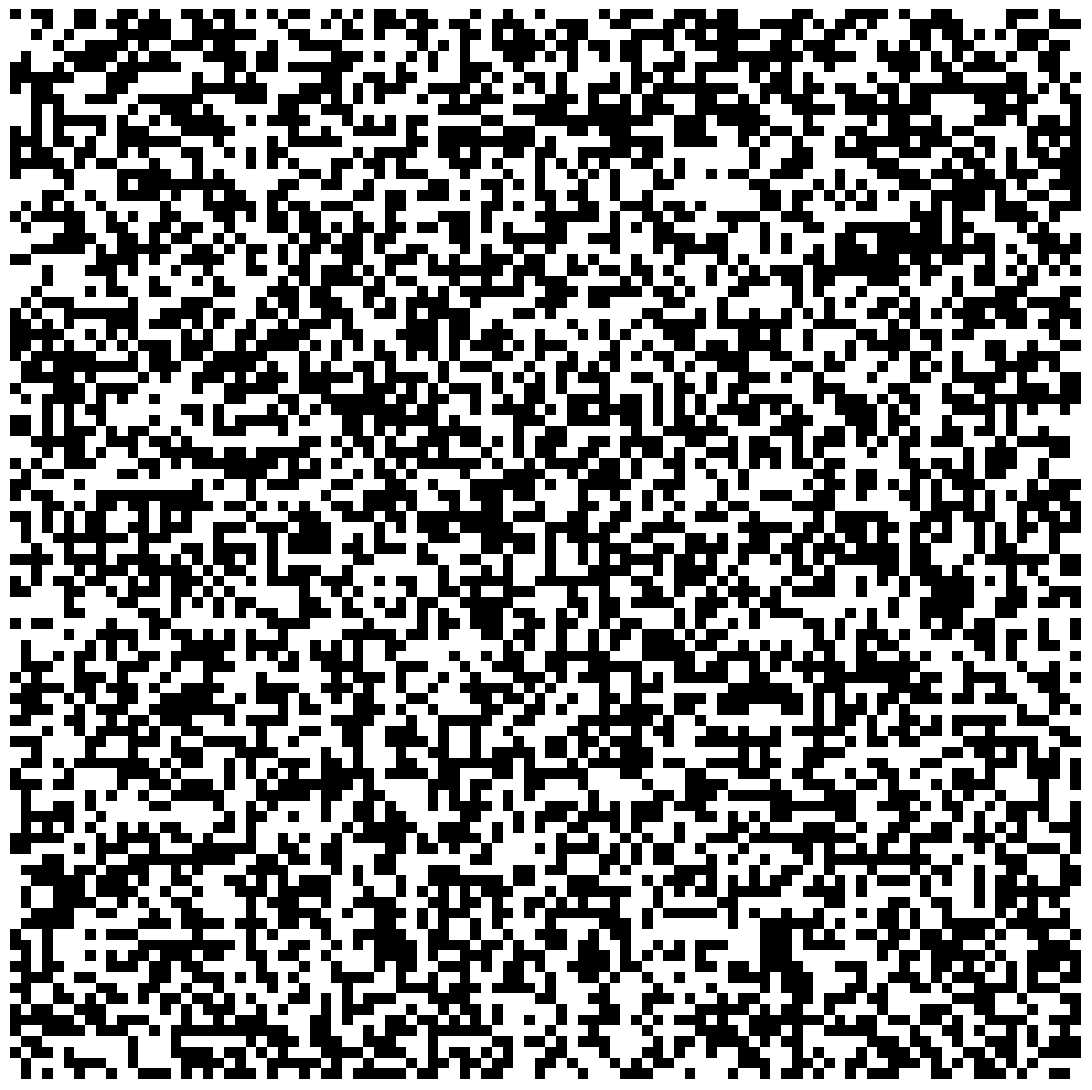
\includegraphics[width=0.65\textwidth]{Figures/verification_melted_lattice.png}
\caption{``Melted'' state of originally ordered lattice at low coldness (high temperature).
Disorder dominates even though $A$-$A$ and $B$-$B$ are energetically favorable relative to $A-B$.}
\label{fig:melted_lattice}
\end{figure}

Second, we show that the method produces highly ordered results when the system is cold and $w_{AB} > w_{AA},w_{BB}$, even if the initial state is entirely random.
Again $d=2 (z=4)$, $L=100$, $x=0.5$,  $w_{AA}=-1$ eV, $w_{BB} = -1$ eV, and $w_{AB} = -0.5$, however now $\beta = 100$ eV$^{-1}$ ($T=116$ K). meaning that the system should energetically prefer minimizing $A$-$B$ contacts.
At such a low temperature, the system should attempt to minmize $A$-$B$ contacts, since they are the least energetically favorable (most positive).
Indeed, even when the lattice is initially random, the system tends to an ordered state with long range order, as shown in Figure \ref{fig:frozen_lattice}
Again, the accompanying convergence plot (Figure \ref{fig:frozen_convergence}) is in the Appendix, and shows 

\begin{figure}[h!]
\centering
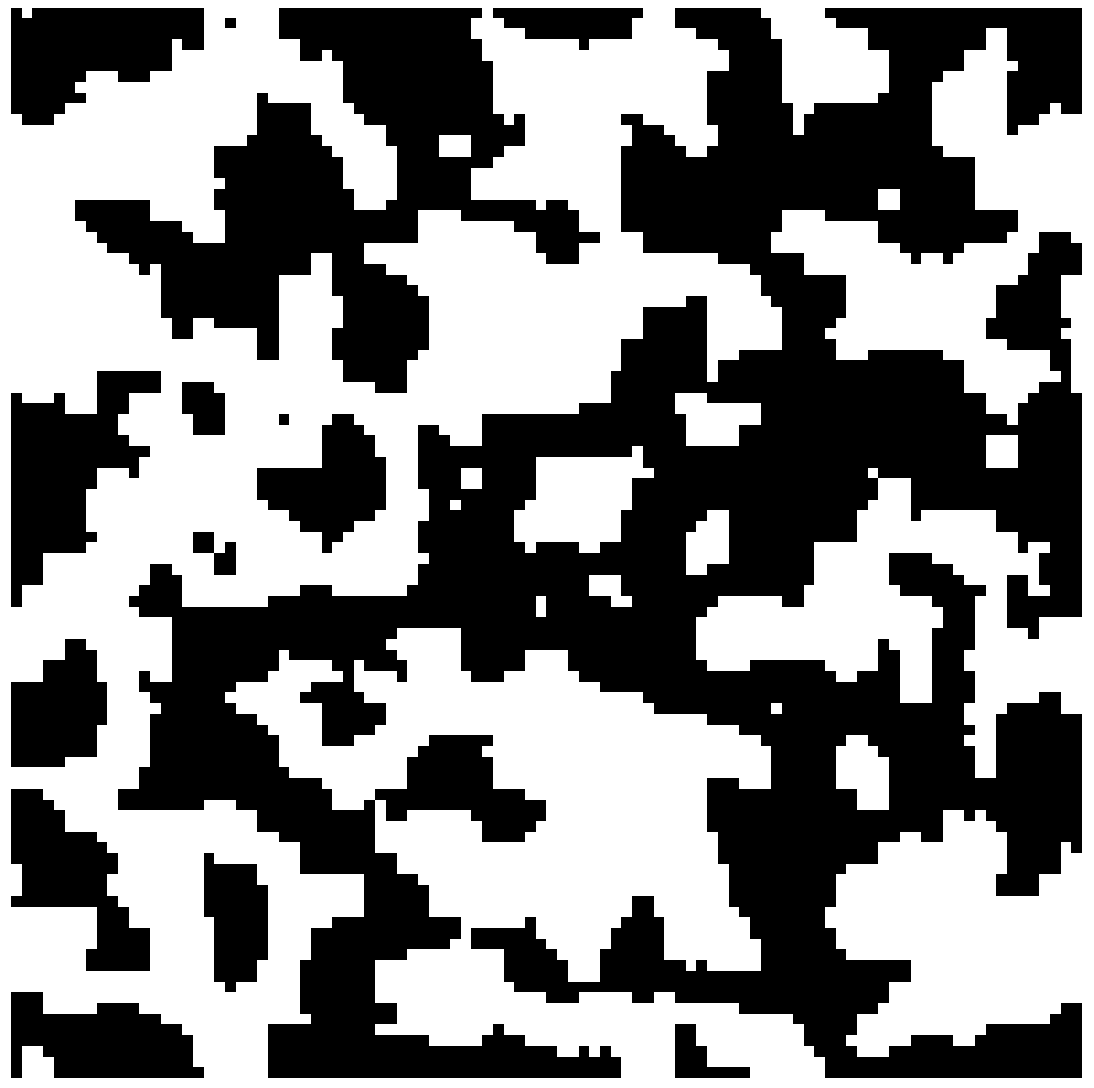
\includegraphics[width=0.65\textwidth]{Figures/verification_frozen_lattice.png}
\caption{``Frozen'' state of originally random lattice at low coldness (high temperature).
Order dominates, following physical intuition.}
\label{fig:frozen_lattice}
\end{figure}

\subsection{One dimensional trends in free parameters}
To visualize the dependence of $\hat{m}_{AB}$ on the system parameters $z,x,\beta,w_{AA},w_{BB},w_{AB}$, we perform plots meshing over each of these parameters, while holding the others constant at $z=4$ ($d = 2$), $x = 0.5$, $\beta = 38.7$ eV$^{-1}$ ($T = 300$ K), $w_{AA} = -1.0$ eV, $w_{BB} = 1.0$ eV, $w_{AB} = -0.5$ eV.
These plots are collected in Figures \ref{fig:m_AB_hat_versus_z} - \ref{fig:m_AB_hat_versus_w_AB}, respectively.

Figure \ref{fig:m_AB_hat_versus_z} shows a nearly linear relationship between $z$ and $\hat{m}_{AB}$ for the test system. \footnote{It is difficult to ascertain the functional form of the dependence with only three points, but this dependence is expected to be linear, as we justify in the next section.} 
Figure \ref{fig:m_AB_hat_versus_x} shows a nonlinear relationship between $z$ and $\hat{m}_{AB}$ for the test system.
Figure \ref{fig:m_AB_hat_versus_beta} displays a sharp transition between just above $\beta = 1$. For very cold systems this configuration minimizes $B$-$B$ interactions in favor of $A$-$B$ interactions, with less preference for $A$-$B$ interactions in system with low coldness (high temperature).
Figure \ref{fig:m_AB_hat_versus_w_AA} shows almost no dependence of $m_{AB}$ on $w_{AA}$, with the present variation likely due to noise.
Figure \ref{fig:m_AB_hat_versus_w_BB} shows another distinct transition-like structure centered around $w_{BB}=0$ eV.
By symmetry it's therefore likely that a similar dependence exists on $w_{AA}$, but perhaps it is not visible due to the asymmetry in the default values of the $w_{XY}$s.
Finally, Figure \ref{fig:m_AB_hat_versus_w_AB}

\begin{figure}[h!]
\centering
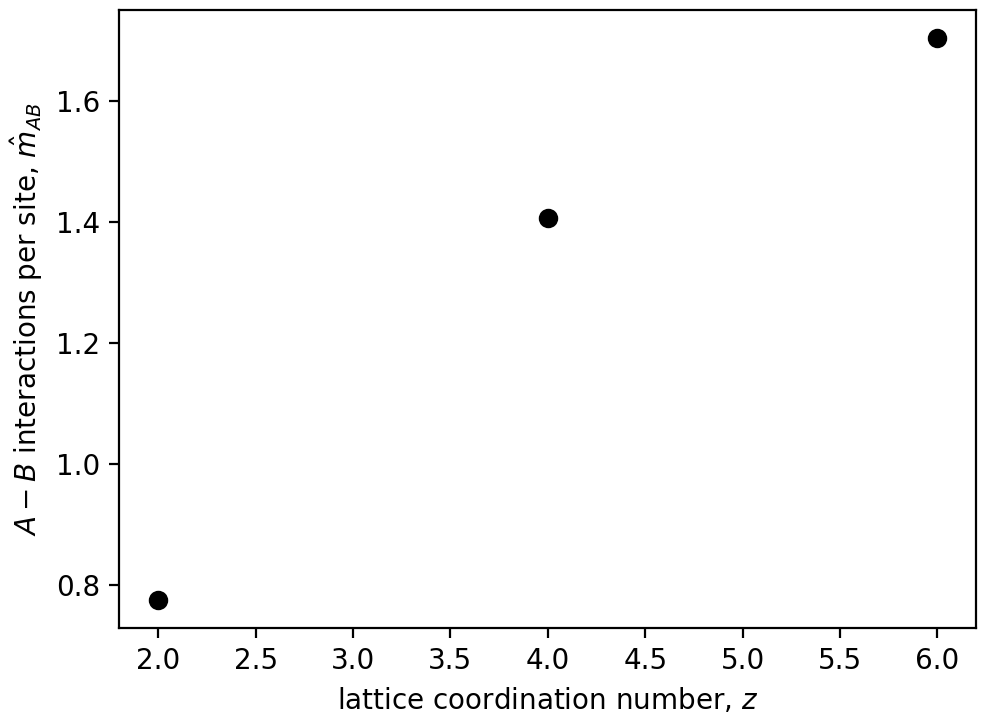
\includegraphics[width=0.65\textwidth]{Figures/m_AB_hat_versus_z.png}
\caption{Number of $A-B$ interactions per site versus lattice coordination number $z$.}
\label{fig:m_AB_hat_versus_z}
\end{figure}

\begin{figure}[h!]
\centering
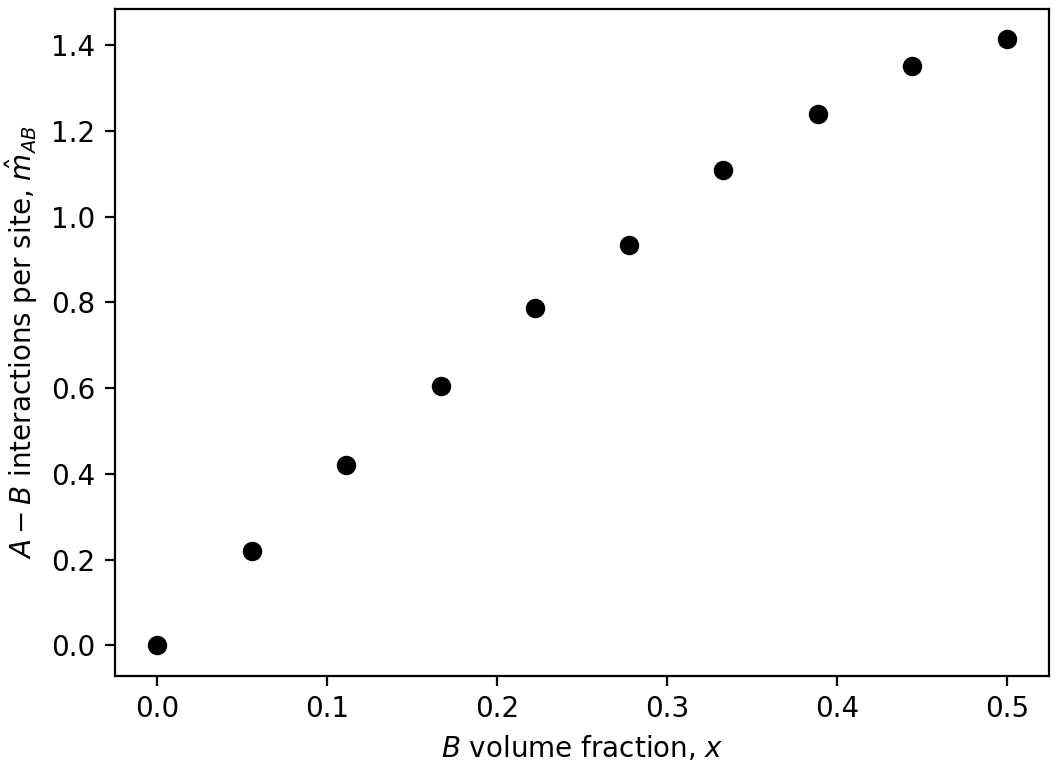
\includegraphics[width=0.70\textwidth]{Figures/m_AB_hat_versus_x.png}
\caption{Number of $A-B$ interactions per site versus $B$ volume fraction $x$.}
\label{fig:m_AB_hat_versus_x}
\end{figure}

\begin{figure}[h!]
\centering
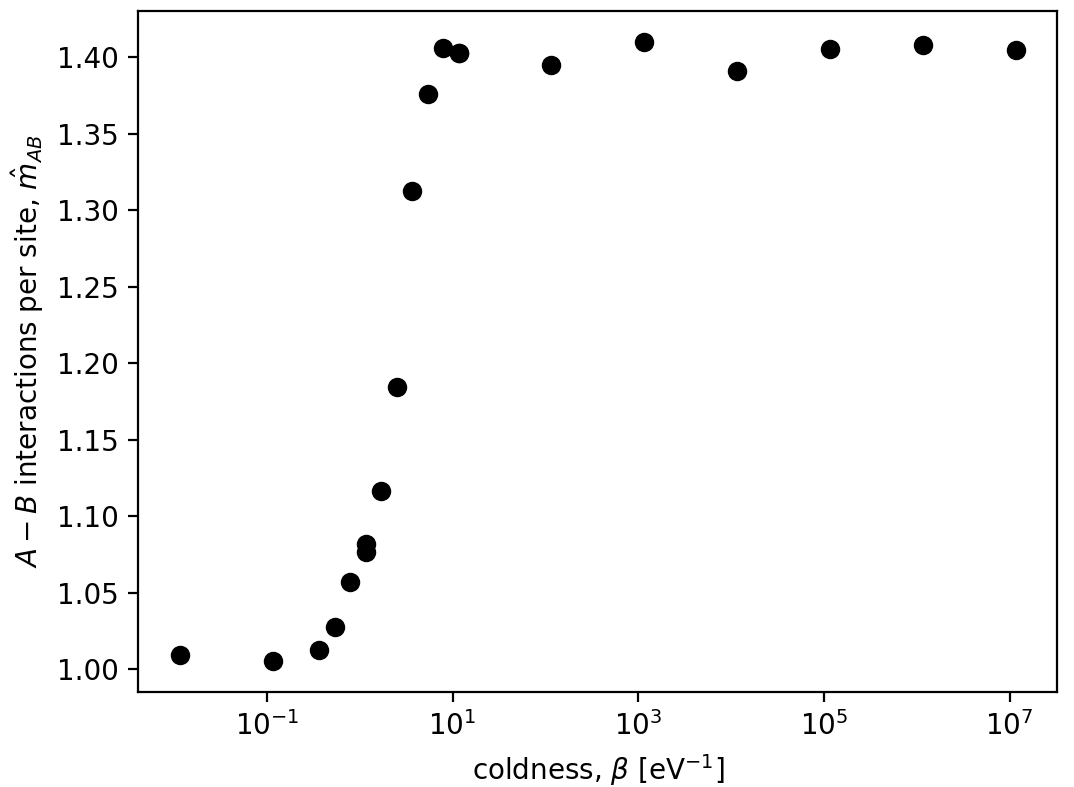
\includegraphics[width=0.67\textwidth]{Figures/m_AB_hat_versus_beta.png}
\caption{Number of $A-B$ interactions per site versus coldness $\beta = \frac{1}{k_B T}$.}
\label{fig:m_AB_hat_versus_beta}
\end{figure}

\begin{figure}[h!]
\centering
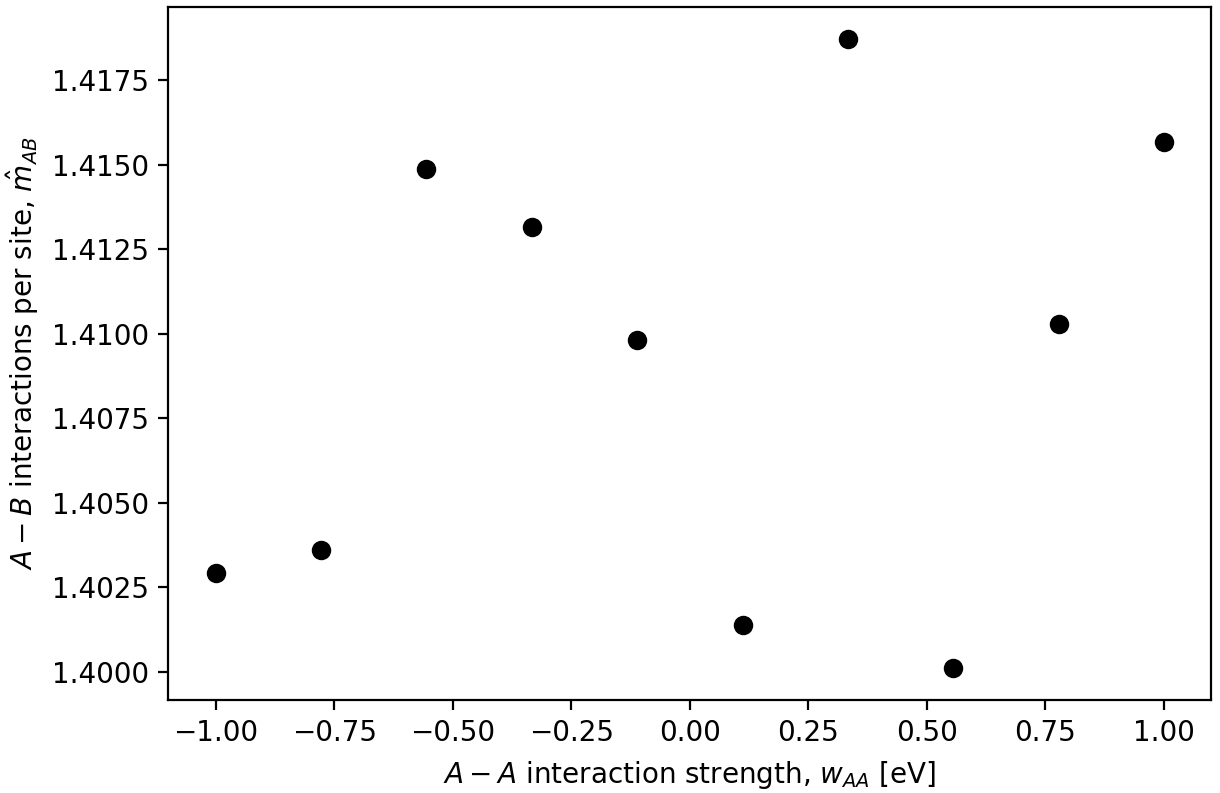
\includegraphics[width=0.70\textwidth]{Figures/m_AB_hat_versus_w_AA.png}
\caption{Number of $A-B$ interactions per site versus $A-A$ interaction strength $w_{AA}$.}
\label{fig:m_AB_hat_versus_w_AA}
\end{figure}

\begin{figure}[h!]
\centering
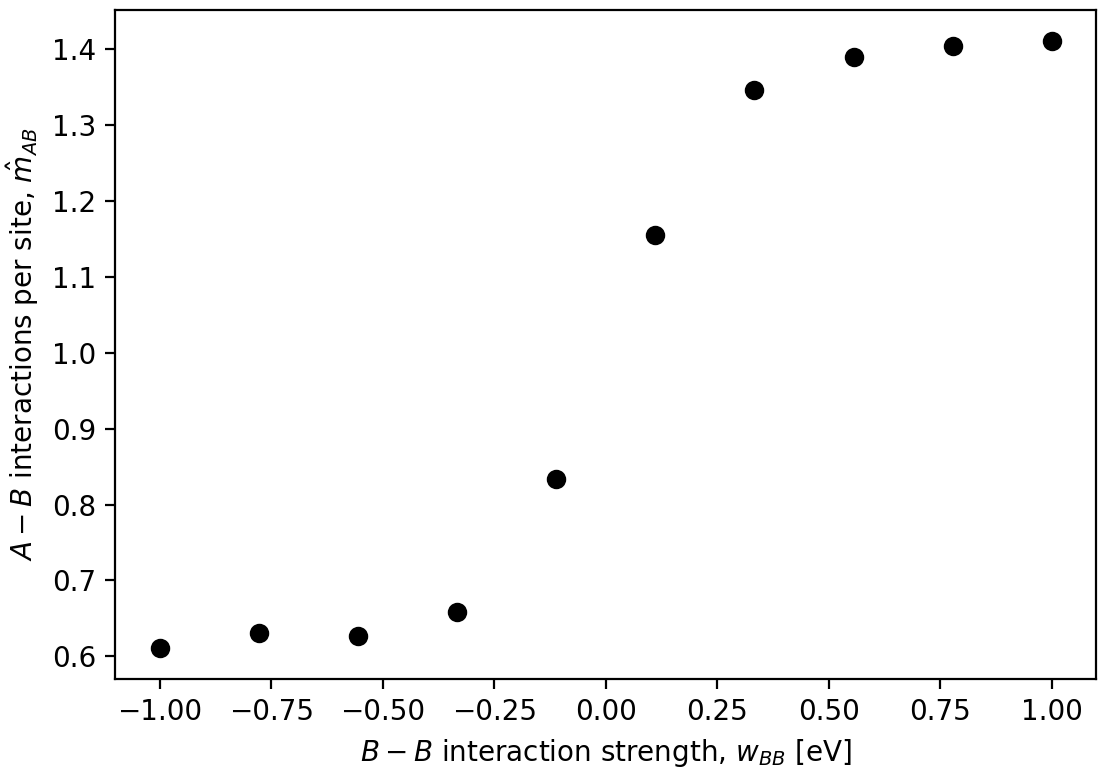
\includegraphics[width=0.70\textwidth]{Figures/m_AB_hat_versus_w_BB.png}
\caption{Number of $A-B$ interactions per site versus $B-B$ interaction strength $w_{BB}$.}
\label{fig:m_AB_hat_versus_w_BB}
\end{figure}

\begin{figure}[h!]
\centering
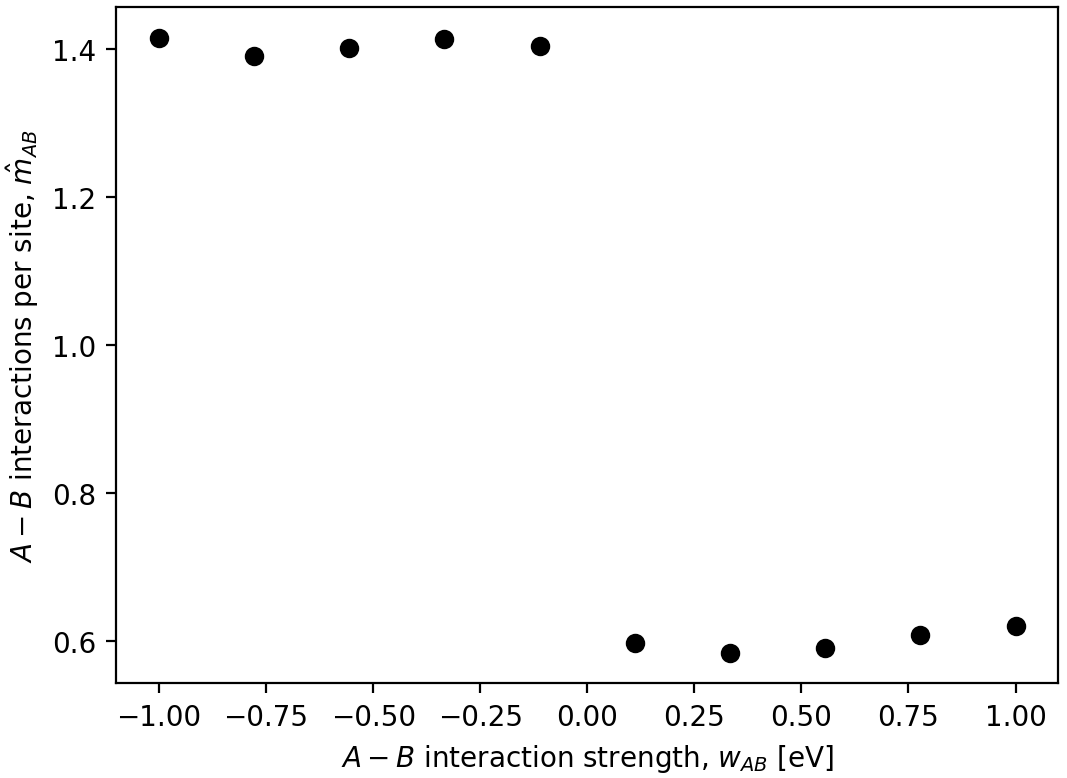
\includegraphics[width=0.70\textwidth]{Figures/m_AB_hat_versus_w_AB.png}
\caption{Number of $A-B$ interactions per site versus $A-B$ interaction strength $w_{AB}$.}
\label{fig:m_AB_hat_versus_w_AB}
\end{figure}

\subsection{Solutions at selected parameter points}
Table \ref{tbl:param_ranges} lists the possible ranges for each of the parameters.
The spatial dimension $d$ covers all common model dimensions for physical systems, the side lattice side length $L$ was chosen to mix small lattices that almost certainly converge to the proper energy with larger lattices that better represent real physical systems.
The $B$ volume fraction $x$ only varies between 0 and 0.5 because the system is symmetric under a relabeling of $A \iff B, w_AA \iff w_BB$.
The interactions strengths were chosen with reference to real physical systems like water with hydrogen bonds of strength -0.24 eV and liquid argon (a common molecular dynamics model system) with equilibrium interaction -0.01 eV \cite{water} \cite{argon}.
The range for temperature $T$ goes from absolute zero to one million Kelvin, which is approximately the point at which the thermal energy scale $k_B T$ is equal to that of the the interaction energy scale defined by $w_XY$.

\begin{center}
\begin{tabular}{c | l | l | l} 
    \hline
    Parameter & Possible Values & Grid spacing & Units \\  \hline
    $d$ & $\mathbb{Z} \in \{1,2,3\}$ & discrete & not applicable \\ \hline
    $L$ & $\mathbb{Z} \in [5,100]$ & discrete & not applicable \\ \hline
    $x$ & $\mathbb{R} \in [0.0,0.5)$ & linear & not applicable \\ \hline
    $T$ & $\mathbb{R} \in [1.0 \times 10^{-3},1.0 \times 10^6]$ & logarithmic & K \\ \hline
    $w_{AA}$ & $\mathbb{R} \in [-1.0, 1.0]$ & linear & eV \\ \hline
    $w_{BB}$ & $\mathbb{R} \in [-1.0, 1.0]$ & linear & eV \\ \hline
    $w_{AB}$ & $\mathbb{R} \in [-1.0, 1.0]$ & linear & eV \\
    \label{tbl:param_ranges}
\end{tabular}
\end{center}



\section{Model Construction}
[overall scheme: generate a bunch of data, then use nonlinear least squares to fit a new function for $\hat{U}$ or $\hat{w}_AB$]

do I fit $\hat{U}$ as function of system parameters, or do I fit $m_{AB}/N$ as a function of system parameters?

\subsection{Model equation construction}
[will need to satisfy some symmetry properties in $x, 1-x$ $w_{AA},w_{AB}$ etc.]

[should have flat multiplier by $z$]

[should have fermi-like transition centered around thermal/interaction transition]

[should reduce to WHAT FORM? in the T=0 case]

[should reduce to the Bragg-Williams approximation for $T \rightarrow \infty$]

The points to which the model was fit include all $2^7$ vertices of the hypercube defined by the extreme values of the parameters in Table \ref{tbl:param_ranges}, in addition to 1000 random points from the interior of the hypercube.
At each of these 1128 points, the energy $\bar{U}$ was computed using the lattice mixture Monte Carlo scheme detailed previously, with termination at $200 \times 10^3$ iterations or $\hat{S}_{\bar{U}} < 5 \times 10^{-5}$ (whichever came first).
For all points the lattice was initialized as a random lattice of the specified $B$ volume fraction $x$.



\newpage
\section{Appendix}
\subsection{Permitted swaps}
Each Monte Carlo step proposes an exchange between two sites in the lattice.
Should each exchange propose swaps between two truly random lattice sites (possibly of the same type), or should each swap be forced to exchange lattice sites of different types.
Of course, swapping two sites of the same type will not change the internal energy, but how does the choice of permitted swaps affect convergence rate and average energy?
Figure \ref{fig:swap} below shows how convergence (in terms of number of Monte Carlo steps) differs for an example case. One can see that while both choice result in the same mean energy, restricting every swap to exchange sites of different types has multiple advantages.
First, the ``transient'' or ``relaxation'' time (where the energy moves toward the equilibrium value) is about half the length, and the same error tolerance is achieved in about 70\% of the steps.
The effect of this choice will be more exaggerated for extremely low and  high volume fractions $x$, where the ``swap any two'' scheme has a high probability of selecting a pair of the same type, whose exchange will not affect the internal energy.

\begin{figure}[h!]
\centering
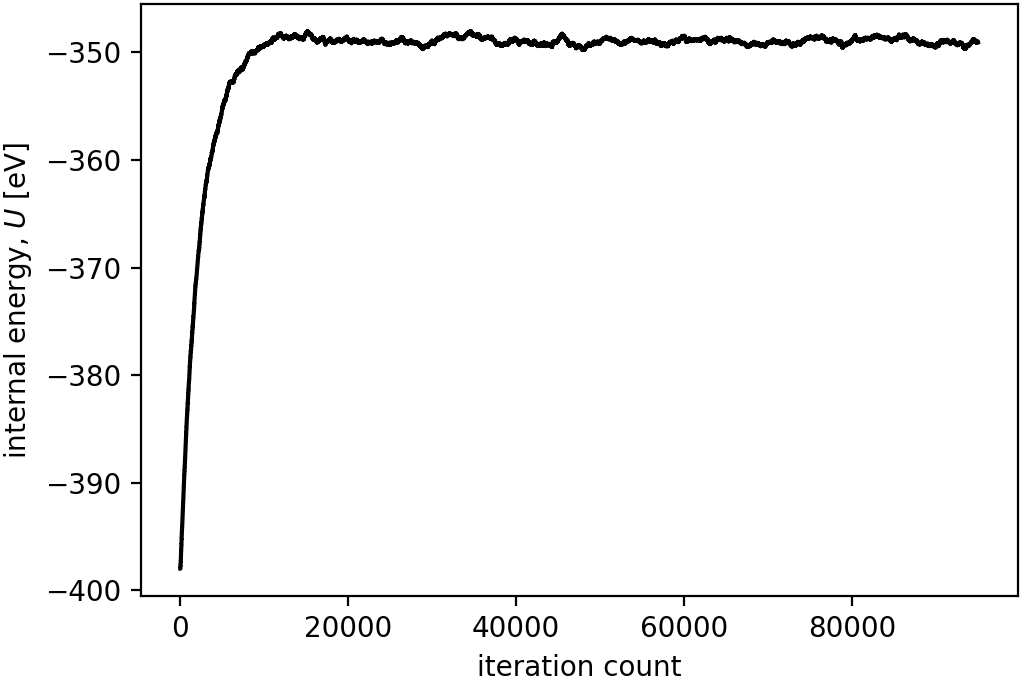
\includegraphics[width=0.49\textwidth]{Figures/swap_any_two_convergence.png}
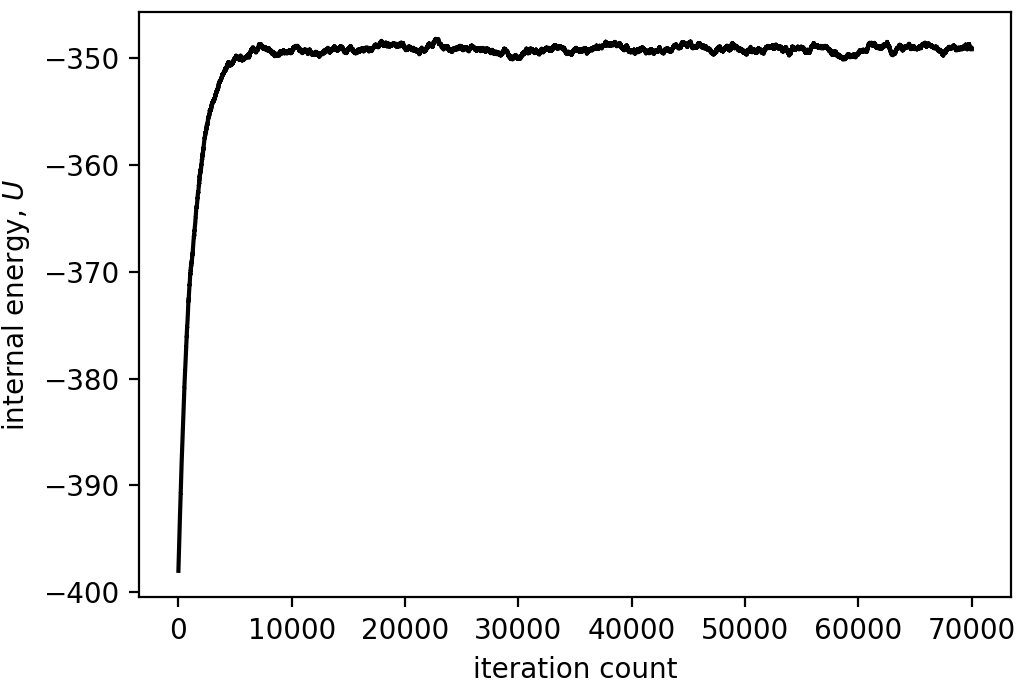
\includegraphics[width=0.49\textwidth]{Figures/swap_A_B_only_convergence.png}
\caption{Internal energy versus iteration with $L=100$, $d=2$, $x=0.5$, $\beta=0.1$, $w_{AA}=w_{AB}=-10 \times 10^{-3},w_{BB} = -30 \times 10^{-3}$ eV; both simulations were run until the percentage error in the mean energy was less than 0.005\%.
The left figure is when swaps may exchange any two sites (independent of their types), while the right figure permits exchanges only between A and B sites.}
\label{fig:swap}
\end{figure}

\subsection{Convergence of verification runs}

\begin{figure}[h!]
\centering
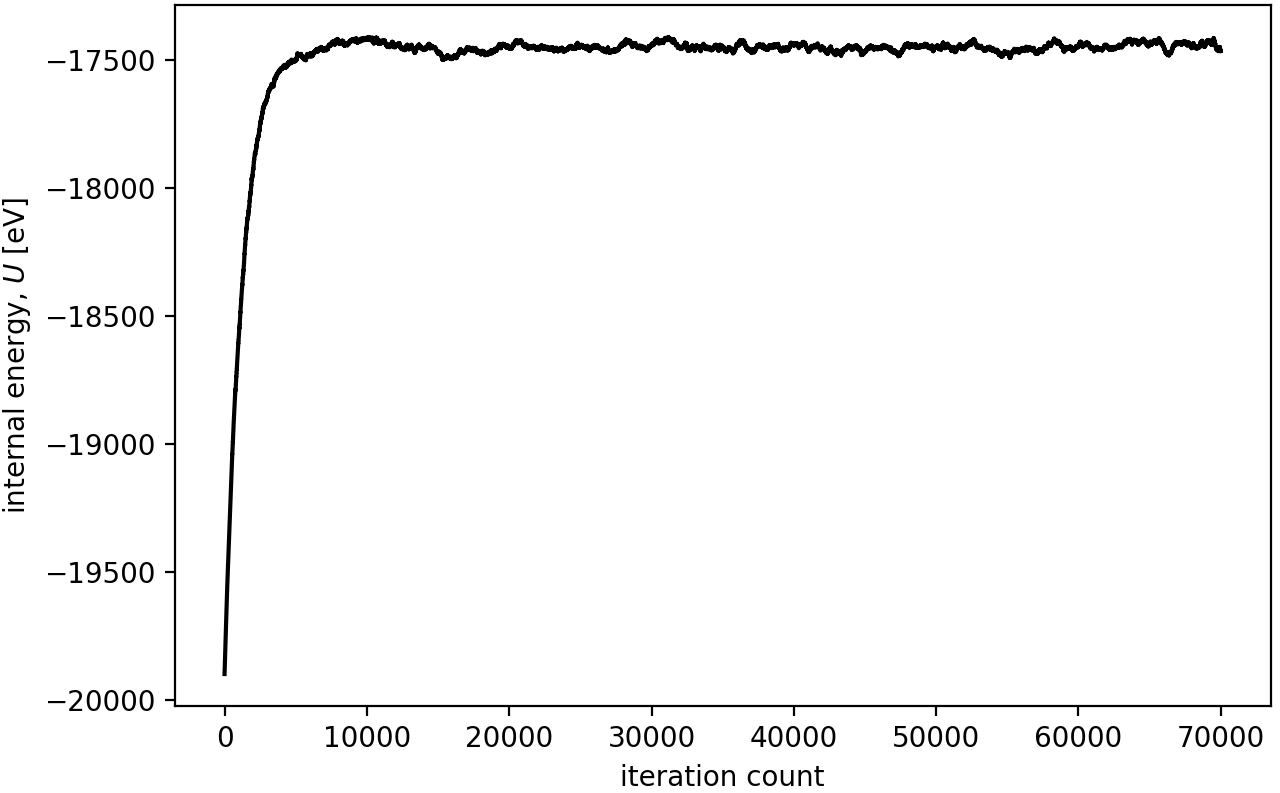
\includegraphics[width=0.80\textwidth]{Figures/verification_melted_convergence.png}
\caption{Energetic convergence to the equilibrium random ``melted'' state of an originally ordered lattice at low coldness (high temperature).
Disorder dominates even though $A$-$A$ and $B$-$B$ are energetically favorable relative to $A$-$B$, and the system starts at in a configuration that minimizes $A$-$B$ contacts.
The larger variations after convergence characterize the low coldness (high temperature).}
\label{fig:melted_convergence}
\end{figure}

\begin{figure}[h!]
\centering
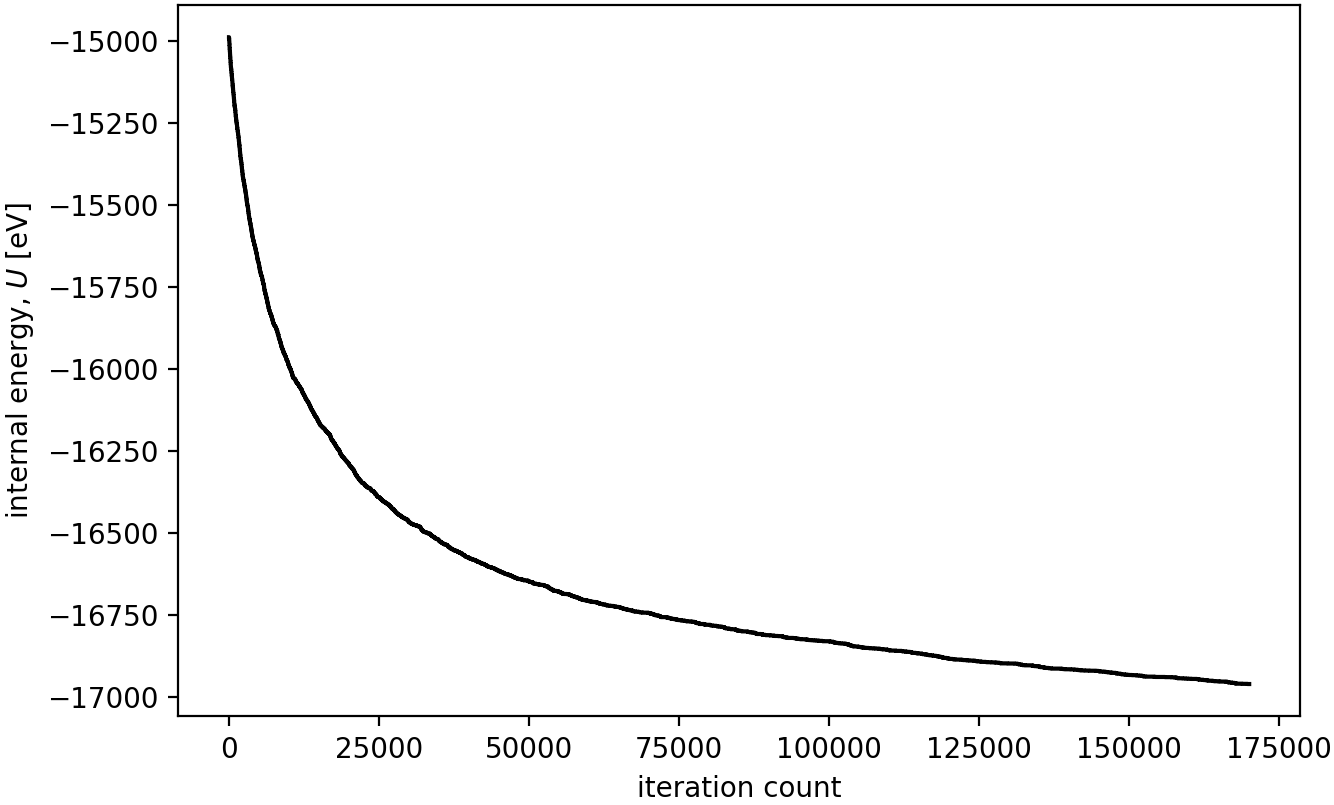
\includegraphics[width=0.80\textwidth]{Figures/verification_frozen_convergence.png}
\caption{Energetic convergence to the equilibrium random ``frozen'' state of an originally random lattice at high coldness (low temperature).
Long range order and structure dominates, driven by energy minimization to reduce the total $A-B$ surface area.
The low variations throughout characterize the high coldness (lower temperature), as the system nearly primarily minimizes energy from step to step.}
\label{fig:frozen_convergence}
\end{figure}


\newpage
\bibliography{references.bib}
References (USE BIBTEX THOUGH)


\end{document}

